% For Monday: 
% - explain why pointers are important
%  - this is the difference between good programmers and mediocre
%    programmers
%  - I have four objectives
%    * read code
%    - write code
%    * self-learn
%    
% Plus an exercise of "human pointers" to implement a Stack
% 
% At the beginning, repeat the stategy re: exercises: all do
% non-stars, some do stars if you finish the non-stars
%
% Representative elections

\section{Interfaces}
\label{sec:interfaces}

Classes in Java have member fields and member methods. The fields are
variables stored inside objects of that class, and contain
information about the object. For example, they can represent the age
of a person or the number of patients in a hospital. The set of all
member fields of an object is usually called the \emph{state} of the
object: they describe how the object \emph{is} at the current moment. 

On the other hand, methods (at least public ones) describe what the
object can do, not what it is. 
For example, a person can say something or a hospital can take
a new patient. The set of (public) methods of a class is usually
called the \emph{behaviour} of the class. 

The behaviour of a class is more important for a programmer than its
state. The state is an implementation detail that can change without
affecting its behaviour, and is usually not important for the task at
hand: this is why fields should be \verb+private+ in most
situations. If I want an object of type \verb+Person+ to say
something, I do not really mind if the person internally uses some
object of type \verb+VocalCord+, or some \verb+Vocoder+, or something
else: I just want the method to do what it is supposed to do. I do not
mind either if a future version of \verb+Person.say(String)+ is
implemented internally in a different way or with different
fields. Actually, it is quite common that the implementation changes
over time (to make it faster, or to use less memory, or to fix bugs)
so I should not worry about it; I should assume it will happen sooner
or later. 

This is why the behaviour of a class is more important than its
state. There are two consequences of this. First, the state should
always be private (we knew that). 
Second, the behaviour must be easy to know and
understand without the need to read the whole code of a class. This
where \emph{interfaces} come in. 

An interface in Java is just a way of showing and explaining the
behaviour of your class. An interface does not contain any information
at all about the implementation or the state of your class. It only
describes some (sometimes all) of the public methods of your
class. Let's see an example: 

\VerbatimInput[frame=single,label=Example of interface]{src/Person.java}

As you can see, the definition of an interface is very similar to the
definition of a class, it is even defined in a java file. 
The difference (and it is a big one!) is that
there are no implementation details at all in the definition of the
interface. It only declares the methods: their names, and their
parameters. Every other detail about the class is left for the class
to be defined. 

There are two more things you may have noticed: 

\begin{itemize}
\item There is no need to say that methods are \verb+public+
  because methods defined on an interface are public by definition.
\item We have introduce a new kind of comments, that start with
  \verb+/**+, end with \verb+*/+ and can span several lines. These
  are called \emph{long comments} and are useful to document your
  code, especially methods, interfaces, and classes. The comments we
  already knew about, that start with \verb+//+ and go to the end of
  the line ---but not to the next line--- are called \emph{short
    comments}. 
\end{itemize}

A class that implements all the methods defined on an interface can
use the reserved keyword \verb+implements+ to mark it. This will tell
the Java compiler that the class \textbf{must} have the methods on the
interface; if it does not, the compiler will complain with an error:
\verb+class is+ \verb+not abstract and+ \verb+does not override+
\verb+abstract method...+ 

Let's see three examples of classes that implement \verb+Person+:

\VerbatimInput[frame=single,label=Implementation 1]{src/AdultPerson.java}

\VerbatimInput[frame=single,label=Implementation 2]{src/KidPerson.java}

As you can see, both \verb+AdultPerson+ and \verb+KidPerson+ implement
the interface \verb+Person+. You can read the keyword
\verb+implements+ as ``is like a''; therefore, \verb+AdultPerson+ 
\emph{is like a} \verb+Person+, and \verb+KidPerson+ \emph{is like a}
\verb+Person+. However, both class implement the interface in
different ways:  

\begin{itemize}
\item \verb+AdultPerson+ uses a member field called \verb+situation+
  while \verb+KidPerson+ uses a member field called
  \verb+position+. This is usually a sign that both classes have been
  coded by different programmers.
\item \verb+KidPerson+ only prints part of the message when the method
  \verb+say(String)+ is called.
\item \verb+KidPerson+ moves slower than \verb+AdultPerson+. The
  latter can move at two different speeds (\verb+run+ and
  \verb+walk+), one of them using more 
  energy than the other. \verb+KidPerson+ has unlimited energy. 
\end{itemize}

From the point of view of a programmer that want to use an object of
type \verb+Person+, all these differences may be irrelevant and
confusing. The programmer just wants an object that moves and says
things. Thanks to the definition (and implementation) 
of Java interfaces, it is perfectly possible to use
objects without knowing their internal details.
Look at the following code: 

\begin{verbatim}
    Person son = new AdultPerson();
    // move in front of mother
    son.move(10);
    // give the message
    son.say("I love you, Mum.");
\end{verbatim}

This code will work exactly the same with \verb+AdultPerson+ and
\verb+KidPerson+. Actually, it will work regardless of the specific class
that is used as long as it
implements the interface \verb+Person+. 

\paragraph{A note about names}
\label{sec:note-about-names}

In Java, the convention is to use short names for interfaces and
longer more-specific names for the classes that implement
them. Interfaces can have names like \verb+Person+ or \verb+Employee+,
while classes have names like \verb+AdultPerson+ and
\verb+PointerManagerEmployee+. 

\paragraph{Conclusion}
\label{sec:conclusion-1}

Interfaces are the way to say what a class \emph{is} and \emph{does},
without saying anything about \emph{how} the class does it. Hiding the
details (i.e.~the actual code) keeps the complexity of the program
lower, resulting in simpler programs that work better and have less
bugs. 

In your programs, make an effort to define interfaces for your classes
(especially the important ones)
and use always the interface instead of the actual class to declare
new variables of the type defined by that class. 

\subsection*{Exercise}
\label{sec:exercise}

Implement a simple class that executes the former code in its main
method. Change the class \verb+AdultPerson+ for \verb+KidPerson+ and
verify that it still compiles and runs. 

\section{Interfaces and data structures}
\label{sec:interfaces-lists}

Interfaces are very important in Java and in any modern
object-oriented programming language. Interfaces allow programmers to
\emph{hide the implementation} of their classes and expose only their
behaviours. This is good because other programmers can use their
classes with minimal effort: they only need to understand the
behaviours, not the full code. Using other programmers' classes (or
your own between different projects) is called \emph{code reuse}, and
saves a lot of effort to programmers (and money to their
companies). For example, you do not need to 
create a new \verb+String+ class every
time you want to write text in your programs: you just use the
\verb+String+ that comes with Java. And you do not need to understand
the code of the class\footnote{The code of all classes in the basic
  Java library is public. You can find it online. Java is free
  software under the GPL license.}, you only need to understand its
behaviour: what \verb+charAt(int)+ does, what
\verb+substring(int,int)+ does, etc. This makes your life much easier
and is good. 

We have seen how dynamic data structures ---like dynamic lists--- 
make it possible to store
unlimited amounts of data in a program (unlike arrays or discrete
variables). Now we are going to see three new special examples of
dynamic lists, and we will define them by using interfaces. 

\subsection{Stacks}
\label{sec:stacks}

We are all familiar with the concept of stacks. When we are putting
books on a box, we usually pile them in stacks; each book is placed 
on top of the
next one, and we can only see the last book we have put, i.e.~the one
on top. When we pile papers on a table we also create stacks. 

Stacks are very important in computing, and are used in many different
contexts. The method-call \emph{stack} (as opposed to the \emph{heap}) 
that stores the variables for each
method in a program is just one well-known example. Every time you
call a method, you create a new level on the stack to store your
variables; while you are in the method, you can only ``see'' the
variables at the top level; when you end the method, those variables are
forgotten and you see the variables on the former level (see
Figure~\ref{fig:stackparameter}).  

\begin{figure}[bthp]
  \centering
  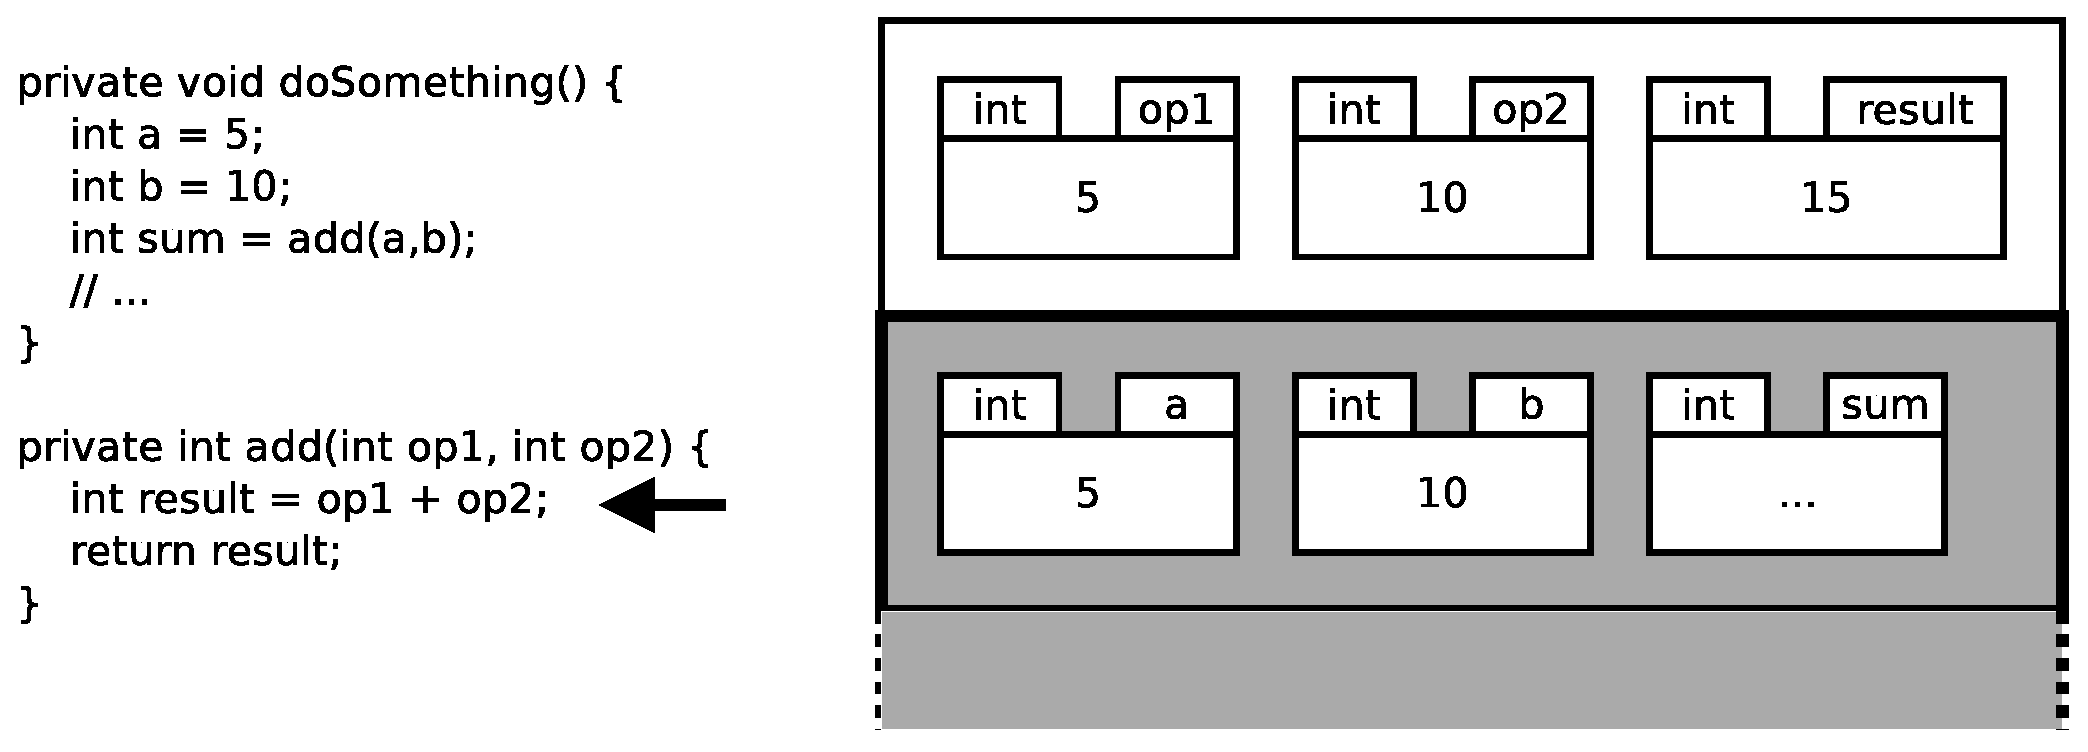
\includegraphics[width=\textwidth]{gfx/parameter-stack}
  \caption{The parameter stack is an example of a stack
    structure. When a method (add) is called, a new level is put on the
    stack to store the parameters and the local variables. While in
    the method, the variables of the other method (a, b, sum) cannot
    be accessed: they are on a different level of the stack, and only
    the most recent one is accessible. Note that if those variables
    were of complex types, their ``boxes'' would be pointers pointing
    to objects in the heap. The arrow marks the current statement.}
  \label{fig:stackparameter}
\end{figure}

In a stack, only the last level is accessible: all former levels are
hidden until the levels on top are removed. This is why stacks are
sometimes called LIFO structures: Last In, First Out. A Stack is
defined by the following methods:

\begin{description}
\item[push($<$type$>$)] puts an element at the top of the stack.
\item[pop() ] removes the element at the top of the
  stack and returns it. 
\item[peek() ] returns the element at the top of the stack, but
  does not remove it from the stack.
\item[isEmpty() ] returns true if there are no elements on the stack,
  false otherwise.
\end{description}

Now have a 
look at the accompanying Java files. 
The first file (\verb+StringStack.java+) is the definition of an
interface for a stack of strings. The next 
one (\verb+ArrayStringStack.java+) is one possible
implementation of this interface based on arrays. The other two files 
(\verb+PointerStringStack.java+, \verb+StringStackNode.java+) are
another possible implementation using linked lists. Which
implementation would you prefer to use? The answer is usually that you
do not mind: \emph{as long as the implementation complies with the
  interface, all implementations are equivalent from your point of
  view}. You can check that both behave exactly the same, regardless
of the number of strings that you \emph{push} on them or 
the order in which you \emph{push} them. You can
use the sample \verb+StringStackScript.java+ file provided or make
your own test.

Sometimes you do mind: maybe one implementation is faster, or uses
less memory, or provides additional methods that are useful for your
program. For instance, the implementation of \verb+PointerStringStack+
has a public method \verb+size()+ that the other implementation does
not. Is this a good addition or an unnecessary burden? The array-based
implementation is usually faster because it does not need to reserve
memory for each element, but sometimes it needs to duplicate the
array, which is slow and uses a lot of memory. Is it more important to
be faster or to use less memory? There is no
general rule that applies to all cases, so a judgement call as a
programmer is always needed. However, judgement is acquired though
practice and experience, and it cannot be expected from a novice
programmer. Therefore, for 
now, it will suffice to know that the rule of thumb is: \emph{work
  with interfaces, not implementations; if the class complies with the
  interface, it is good enough}. You have an example in
\verb+StringStackScript.java+: the name of the class is only used to
instantiate (i.e.~create the object); after that, we only use the name
of the interface. We do not need anything else. 

\subsection{Queues}
\label{sec:queues}

Queues are, in a way, the opposite of stacks. Stacks are LIFO
structures, queues are FIFO structures: First In, First 
Out (Figure~\ref{fig:fifolifo}). It is the
same idea as the queues at the airport or at the supermarket. 

\begin{figure}[hbtp]
  \centering
  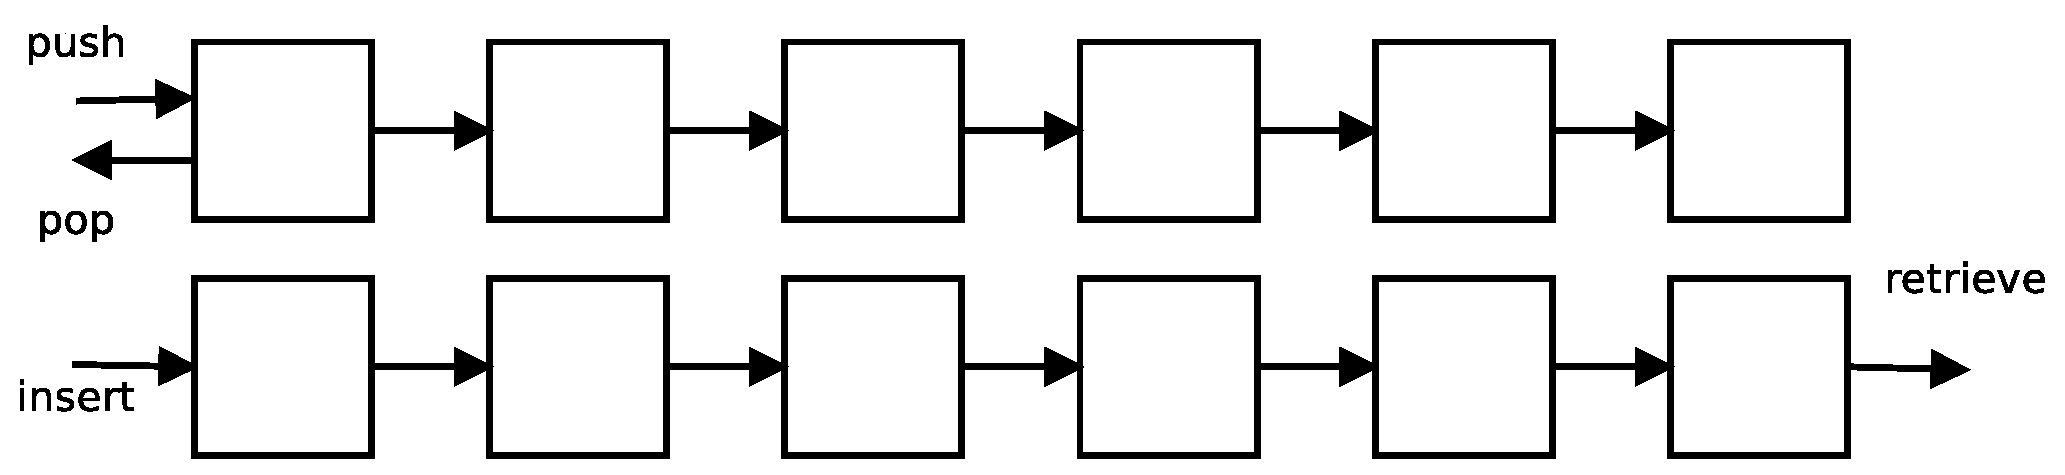
\includegraphics[width=\textwidth]{gfx/fifo-lifo}
  \caption{Stacks are LIFO. Queues are FIFO.}
  \label{fig:fifolifo}
\end{figure}

The same as stacks, queues are very popular data structures that you
can find everywhere in computing: your wi-fi connection has a queue of
bytes to send on the air, the web server at \verb+www.bbk.ac.uk+ has a
queue of requests from web browsers, and your hard disk has a queue of
petitions to read or write on it. 

Queues are defined by the following interface: 

\begin{description}
\item[insert($<$type$>$)] adds an element to the queue.
\item[retrieve() ] removes an element from the queue.
\end{description}

It is common that queues provide a method \verb+getSize()+ that
returns the current size of the queue. 
Some queues may have a
maximum size\footnote{Strictly speaking, all queues are limited: even
  ``unbounded'' queues cannot be larger than the memory available on
  the machine.} and provide a 
method \verb+getMaxSize()+ that returns the maximum size possible, so
that other classes know in order to prevent data
loss. For example, when you hear in the news that a website has
suffered a Distributed Denial of Service attack (DDoS) that means that
a lot of computers are issuing simultanenous requests to the same web
server until its queue is full and all new requests are ignored.

\subsection{Maps}
\label{sec:map}

When a list has many elements, it can take a long time to find the
element you are looking for. In order to reduce the time needed to
delete or find an element in long lists we have \emph{maps}.

A map is a special kind of data structure that links some piece of
data, called the \emph{key}, with one or more pieces of data, called
the \emph{value} or \emph{values}. The contact agenda in your mobile
phone is an example of a map: it maps names to phone numbers. Other
examples of maps are address books that link addresses with people,
building maps that link floors with companies, and keyboards that link
physical keys with letters and symbols. 

A map can link each key with one value or more. Depending on the
application, one behaviour may be more appropriate than the
other. Maps that link exactly one value to every key are sometimes
called \emph{dictionaries}. 

Maps are useful in computing because we want programs to run fast but
lists are usually very long; think of the number of files on your
computer; the number of past and future patients in a big hospital; or
the number of citizens in the Goverment's tax computers. If a map can
link each key (like an ID) to one value, looking for it is very
fast. Even if a map links a key to many different values (like the
initial of a family name) it reduces the search time
considerably. Maps that link one key to many values are sometimes
called \emph{hash tables}. This is because they use a \emph{hash}
function that reduces the whole search space (e.g.~every possible
family name in the world) to a reduced one (e.g.~the letters of the
alphabet). One simple hash function is the modulo operator: it reduces
every possible integer in the world to a reduced set of integers. Hash
functions are important in many fields of computing ---like computer
security--- and the search of good hash functions is an active field of
research. 

A map is defined by the following interface: 

\begin{description}
\item[put($<$keytype$>$, $<$valuetype$>$)] adds a new element to the
  map, associated with a key; depending on whether the key has already
  been used, and whether the map allows more than one value per key,
  this method can return different types. 
\item[get($<$keytype$>$) ] gets the value associated with that key.
\item[isEmpty() ] returns true if there are no elements on the stack,
  false otherwise.
\end{description}




%              interfaces
%              queues and stacks, 
%              trees, binary and non-binary trees, 
%              basics of memory allocation, gargage collection, 


%%% Local Variables:
%%% mode: latex
%%% TeX-master: "main"
%%% End:
